\section{Durchführung}
\label{sec:Durchführung}

Die Dampfdruckkurve wird in zwei Bereichen bestimmt.
Einmal wird in einem Bereich zwischen ca. \qty{30}{\milli\bar} und \qty{1000}{\milli\bar} gemessen.
Danach in einem Hochdruckbereich von \qty{1}{\bar} bis \qty{15}{\bar} gemessen.
Im folgenden werden die einzelnen Methoden erläutert.

\subsection{Messungen im Niedrigdruckbereich unter 1 bar} % (fold)
\label{sub:M_Niedrigdruckbereich}
Im Druckbereich bis $\qty{1}{\bar}$ kann der Aufbau in \autoref{fig:Abb_3} genutzt werden.
\begin{figure}[H]
    \centering
    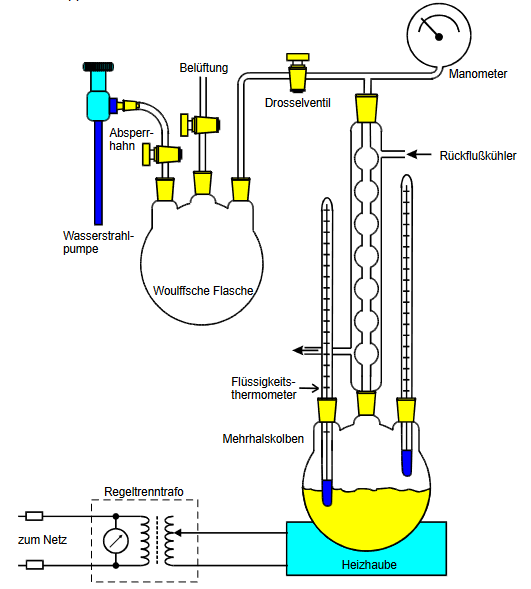
\includegraphics[width=0.7\textwidth]{build/Abb_3.PNG}
    \caption {Aufbau zur Messung unter $\qty{1}{\bar}$.\cite{V203}}
    \label{fig:Abb_3}
\end{figure}
Vor der Messung muss der Aufbau evakuiert werden.
Dies erfolgt mit Hilfe einer Wasserstrahlpumpe. Dafür muss das Belüftungsventil geschlossen sein und der Absperrhahn und das Drosselventil werden geöffnet.
Es wird solange evakuiert, bis der Druck nicht weiter sinkt. 
Die Messung beginnt erst, wenn der Enddruck der Evakuierung erreicht wird.
Dieser ist unter anderem abhängig von der Leitungswassertemperatur.
Die Woulffsche Flasche im Aufbau verhindert, dass kaltes Wasser nach dem Abstellen der Wasserstrahlpumpe in die erhitzte und evakuiert Apparatur eindringt.
Bevor die Wasserstrahlpumpe abgestellt wird, muss der Absperrhahn geschlossen werden.
Nun beginnt die Messung.
Der Mehrhalskolben mit der Flüssigkeit wird erhitzt und der Rückflusskühler wird während der gesamten Messung mit Leitungswasser durchflossen.
Dies dient dazu, dass die aufsteigenden Dämpfe kondensieren und nicht ins Manometer gelangen, welches den Druck misst.
Während der Messung wird die Temperatur am Thermometer abgelesen und zu den Drücken in eine Tabelle geschrieben.
Die Menge des Kühlwassers muss bei steigender Temperatur verringert werden.
Die Messung endet, wenn der Druck im Inneren der Apparatur auf $\qty{1000}{\milli\bar}$ gestiegen ist.
% subsection M_Niedrigdruckbereich (end)

\subsection{Messungen im Hochdruckbereich über 1 bar} % (fold)
\label{sub:M_Hochdruckbereich}
Im Druckbereich ab \qty{1}{\bar} muss ein anderer Aufbau benutzt werden, wie zum Beispiel \autoref{fig:Abb_4}.
\begin{figure}[H]
    \centering
    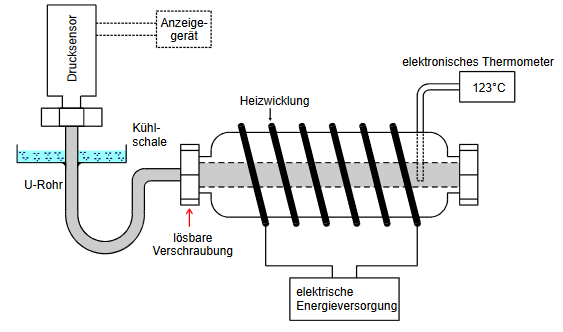
\includegraphics[width=0.7\textwidth]{build/Abb_4.PNG}
    \caption {Aufbau zur Messung über $\qty{1}{\bar}$.\cite{V203}}
    \label{fig:Abb_4}
\end{figure}
Diese Apparatur besteht aus einem durchbohrten Stahlbolzen, in dessen Hohlraum sich destilliertes und entgastes Wasser befindet,
einem U-Rohr, einem Barometer und einem Thermometer.
Außerdem befindet sich unter dem Stahlzylinder eine Heizwicklung, die den Stahlbolzen langsam aufheizt.
Die Heizung wird angeschlatet und die Messung beginnt, sobald das Barometer $\qty{1}{\bar}$ anzeigt.
Während der Messung werden die Temperatur und der Druck abgelesen und in einer Tabelle notiert.
Die Messung endet wenn das Barometer $\qty{15}{\bar}$ anzeigt.
% subsection Messungen im Hochdruckbereich über \ (end)